\section{Pendahuluan}
\subsection{Latar Belakang}
Di era globalisasi ini dimana dunia semakin terhubung satu sama lain, jaringan komputer menjadi salah satu pilar penting dalam kehidupan sehari-hari. Hampir semua aktivitas di dunia modern, baik itu di rumah, universitas, atau bahkan perusahaan, membutuhkan jaringan untuk komunikasi antar perangkat yang digunakan. Tanpa jaringan komputer, pertukaran informasi antar perangkat akan sangat terbatas, bahkan hampir tidak mungkin dilakukan. Oleh karena itu, pemahaman yang baik tentang cara kerja jaringan komputer sangatlah penting, terutama dalam dunia profesional yang semakin bergantung pada teknologi.
Namun, dalam membangun jaringan komputer yang efisien seringkali menghadapi tantangan, seperti bagaimana pengalokasian IP address yang tepat, menghindari pemborosan, dan memastikan komunikasi antar perangkat berjalan lancar. Selain itu, pemilihan dan penerapan protokol komunikasi yang sesuai juga menjadi penting untuk menjaga keamanan dan stabilitas jaringan.
Praktikum ini sangat penting dilakukan karena dengan adanya praktikum ini diiharapkan mahasiswa memahami dan menerapkan konsep-konsep dasar jaringan, seperti IP address, subnetting, dan konfigurasi router.
Penerapan dari hasil praktikum ini di dunia nyata sangat luas karena jaringan komputer mendukung berbagai teknologi seperti IoT, smart home, dan aplikasi bisnis berbasis cloud. Pengelolaan jaringan yang baik juga diperlukan dalam dunia industri dan kehidupan sehari-hari, misalnya untuk menghubungkan perangkat melalui Wi-Fi.
\subsection{Dasar Teori}
\begin{enumerate}
	\item Jaringan Komputer 
	
	Jaringan komputer adalah sekumpulan perangkat yang saling terhubung untuk berbagi data dan sumber daya. Jaringan ini memungkinkan berbagai perangkat untuk berinteraksi dan bertukar informasi secara efisien. Jenis-jenis jaringan komputer yang umum digunakan antara lain LAN (Local Area Network), WAN (Wide Area Network), dan MAN (Metropolitan Area Network). LAN digunakan untuk jaringan dalam area kecil, WAN untuk jaringan yang mencakup area yang lebih luas, dan MAN untuk jaringan antar gedung dalam satu kota.
	\item IP Address
	
	IP Address adalah alamat unik yang digunakan untuk mengidentifikasi perangkat dalam jaringan. Setiap perangkat yang terhubung ke jaringan memerlukan IP address untuk bisa berkomunikasi dengan perangkat lain dalam jaringan tersebut. Ada dua jenis utama IP address yang digunakan dalam jaringan komputer:
	\begin{itemize}
		 \item IP Statis adalah alamat yang tetap dan tidak berubah selama perangkat tersebut terhubung ke jaringan. IP statis biasanya digunakan pada server, perangkat yang diakses secara jarak jauh, atau perangkat yang membutuhkan koneksi stabil dan konsisten.
		 \item IP Dinamis adalah alamat yang diberikan secara otomatis oleh server DHCP (Dynamic Host Configuration Protocol). IP dinamis ini dapat berubah setiap kali perangkat terhubung kembali ke jaringan atau setiap kali perangkat tersebut di-restart.
	\end{itemize}
Terdapat pula subnetting yang mana merupakan proses pembagian sebuah jaringan besar menjadi beberapa jaringan lebih kecil (subnet). Proses ini berguna untuk mengoptimalkan penggunaan alamat IP dan meningkatkan efisiensi serta keamanan jaringan. Dalam subnetting, alamat IP dibagi menjadi dua bagian utama: Network ID, yang mengidentifikasi jaringan tempat perangkat berada, dan Host ID, yang mengidentifikasi perangkat dalam jaringan tersebut.
	\item Protokol Jaringan 
	
	Protokol adalah sekumpulan aturan yang mengatur cara komunikasi antara perangkat dalam jaringan komputer. Tanpa protokol, perangkat dalam jaringan tidak akan bisa saling mengerti dan bertukar data. Beberapa protokol yang paling sering digunakan dalam jaringan komputer adalah:
	\begin{itemize}
		 \item TCP/IP (Transmission Control Protocol/Internet Protocol): Merupakan pasangan protokol yang paling penting dalam jaringan komputer. TCP memastikan bahwa data dikirimkan dengan urutan yang benar dan tanpa ada yang hilang, sedangkan IP mengatur pengalamatan dan rute data ke tujuan yang benar.
		 \item HTTP (Hypertext Transfer Protocol) dan HTTPS (Hypertext Transfer Protocol Secure): HTTP digunakan untuk komunikasi web standar, sedangkan HTTPS adalah versi HTTP yang lebih aman dengan enkripsi, sering digunakan dalam transaksi online untuk melindungi data pribadi.
		 \item FTP (File Transfer Protocol): FTP digunakan untuk mentransfer file antara perangkat dalam jaringan. Protokol ini memungkinkan pengiriman file dalam berbagai format antara server dan pengguna.
		 \item DHCP (Dynamic Host Configuration Protocol): Protokol ini digunakan untuk memberikan alamat IP secara otomatis kepada perangkat yang terhubung ke jaringan. DHCP memungkinkan perangkat untuk mendapatkan alamat IP tanpa harus dikonfigurasi secara manual.
	\end{itemize}
	\item Routing dalam Jaringan
	
	Routing adalah proses memilih jalur yang harus ditempuh oleh data untuk sampai ke tujuan. Dalam jaringan yang lebih besar, ada lebih dari satu jalur untuk mengirimkan data, dan router bertugas memilih jalur terbaik. Ada dua jenis routing yang umum digunakan:
	\begin{itemize}
		 \item Routing Statis: Pada routing statis, administrator jaringan secara manual menentukan rute yang harus diambil oleh data. Rute ini bersifat tetap, dan hanya berubah jika dilakukan perubahan secara eksplisit pada konfigurasi jaringan.
		 \item Routing Dinamis: Routing dinamis menggunakan protokol routing seperti RIP (Routing Information Protocol) atau OSPF (Open Shortest Path First) agar secara otomatis dapat memperbarui dan memilih jalur terbaik berdasarkan kondisi jaringan yang berubah. Protokol ini memungkinkan router saling bertukar informasi tentang kondisi jaringan, sehingga rute data dapat berubah secara otomatis jika ada perubahan dalam jaringan.
	\end{itemize}

	\item Subnet Mask dan Prefix

	Subnet Mask adalah angka yang digunakan untuk membagi alamat IP menjadi dua bagian utama: Network ID dan Host ID. Mask ini mengidentifikasi bagian mana dari alamat IP yang digunakan untuk jaringan dan bagian mana yang digunakan untuk perangkat dalam jaringan tersebut. Misalnya, dengan subnet mask 255.255.255.0 (atau prefix /24), 24 bit pertama digunakan untuk Network ID, sementara 8 bit terakhir digunakan untuk Host ID. 
	
	Terdapat pula metode CIDR (Classless Inter-Domain Routing) yaitu metode pengalokasian alamat IP yang lebih fleksibel daripada metode tradisional berdasarkan kelas (A, B, C). CIDR memungkinkan penggunaan prefix yang lebih panjang atau lebih pendek untuk mendefinisikan ukuran subnet secara lebih tepat.

	\item Keamanan Jaringan
	
	Keamanan jaringan sangat penting untuk memastikan data dan perangkat yang terhubung ke jaringan terlindungi dari ancaman seperti peretasan, penyadapan, dan akses tidak sah. Beberapa teknik yang digunakan untuk meningkatkan keamanan jaringan antara lain:
	\begin{itemize}
		\item Firewall: Sistem yang digunakan untuk memonitor dan mengontrol lalu lintas data yang masuk dan keluar dari jaringan berdasarkan aturan yang ditentukan.
		\item SSL/TLS (Secure Sockets Layer/Transport Layer Security): Protokol enkripsi yang digunakan untuk menjaga keamanan data yang dikirimkan melalui internet. HTTPS adalah salah satu contoh penggunaan SSL/TLS untuk mengamankan komunikasi web.
	\end{itemize}

	\item Pengkabelan LAN dan Crimping
	
Crimping adalah proses memasang konektor RJ45 pada kabel UTP untuk membentuk kabel yang digunakan dalam jaringan lokal (LAN). Koneksi kabel ini penting agar perangkat dapat terhubung dan berkomunikasi satu sama lain dalam jaringan. Terdapat dua jenis pengkabelan yang umum digunakan:
\begin{itemize}
	\item Straight-Through: Digunakan untuk menghubungkan perangkat yang berbeda jenis, seperti komputer ke switch atau router.
	\item Crossover: Digunakan untuk menghubungkan perangkat yang sama jenisnya, seperti komputer ke komputer atau router ke router.
\end{itemize}
\end{enumerate}
%===========================================================%
\section{Tugas Pendahuluan}
\begin{enumerate}
	\item Rentang IP address dan prefix (CIDR) serta total Subnet
	\begin{itemize}
		\item Departemen Produksi
		\begin{enumerate}
		\item Jumlah Perangkat: 50 perangkat
		\item Subnet yang dibutuhkan: Untuk menampung 50 perangkat, membutuhkan setidaknya 64 alamat IP, karena 64 adalah kelipatan dua terdekat yang lebih besar dari 50.
		\item Prefix CIDR: /26 (Subnet mask: 255.255.255.192) yang menyediakan 64 alamat IP.
		\item Rentang IP: Misalnya menggunakan 192.168.1.0/26. Ini memberikan alamat dari 192.168.1.0 hingga 192.168.1.63

		Network address: 192.168.1.0
	
		Broadcast address: 192.168.1.63
		
		Alamat yang bisa digunakan: 192.168.1.1 hingga 192.168.1.62
	\end{enumerate}
		\item Departemen Administrasi
		\begin{enumerate}
		\item Jumlah Perangkat: 20 perangkat
		\item Subnet yang dibutuhkan: Untuk menampung 20 perangkat, kita membutuhkan setidaknya 32 alamat IP
		\item Prefix CIDR: /27 (Subnet mask: 255.255.255.224) yang menyediakan 32 alamat IP.
		\item Rentang IP: Misalnya menggunakan 192.168.1.64/27
		Memberikan alamat dari 192.168.1.64 hingga 192.168.1.95.

		Network address: 192.168.1.64
	
		Broadcast address: 192.168.1.95
		
		Alamat yang bisa digunakan: 1192.168.1.65 hingga 192.168.1.94
	\end{enumerate}
	\item Departemen Keuangan
		\begin{enumerate}
		\item Jumlah Perangkat: 10 perangkat
		\item Subnet yang dibutuhkan: Untuk menampung 10 perangkat, kita membutuhkan setidaknya 16 alamat IP.
		\item Prefix CIDR: /28 (Subnet mask: 255.255.255.240) yang menyediakan 16 alamat IP.
		\item Rentang IP: Misalnya menggunakan 192.168.1.96/28. Memberikan alamat dari 192.168.1.96 hingga 192.168.1.111

		Network address: 192.168.1.96
	
		Broadcast address: 192.168.1.111
		
		Alamat yang bisa digunakan: 192.168.1.97 hingga 192.168.1.110
	\end{enumerate}
		\item Departemen RnD
		\begin{enumerate}
		\item Jumlah Perangkat: 100 perangkat
		\item Subnet yang dibutuhkan: Untuk menampung 100 perangkat, membutuhkan setidaknya 128 alamat IP
		\item Prefix CIDR: /25 (Subnet mask: 255.255.255.128) yang menyediakan 128 alamat IP.
		\item Rentang IP: Misalnya kita menggunakan 192.168.1.128/25. Ini memberikan alamat dari 192.168.1.128 hingga 192.168.1.255
		Network address: 192.168.1.128
	
		Broadcast address: 192.168.1.255
		
		Alamat yang bisa digunakan: 192.168.1.129 hingga 192.168.1.254
	\end{enumerate}
	\end{itemize}
	\item Topologi sederhana yang menunjukkan bagaimana router akan menghubungkan semua subnet.
\begin{figure}[h]
    \begin{center}
        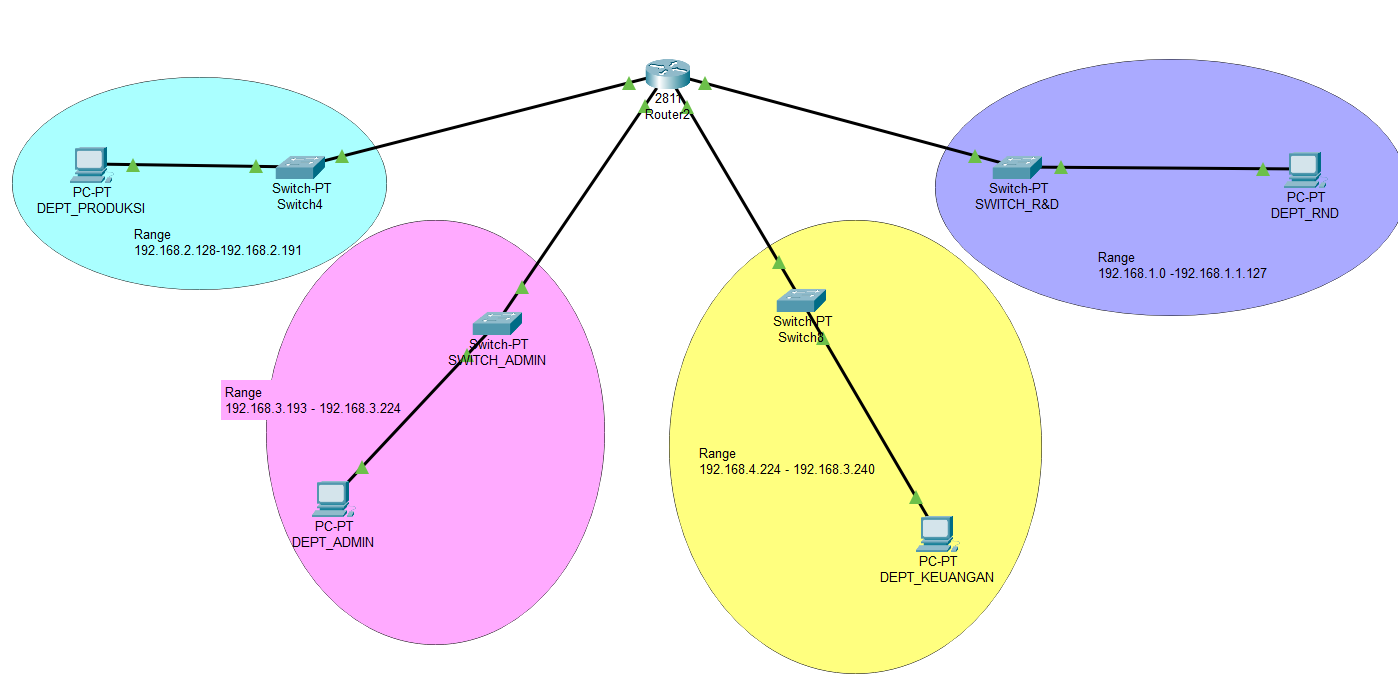
\includegraphics[scale=0.36]{P1/img/tupenp1.png}
        \caption{Topologi Sederhana Menggunakan Cisco}
        \label{fig:tupenp1}
    \end{center}
\end{figure}

\begin{figure}[h]
    \begin{center}
        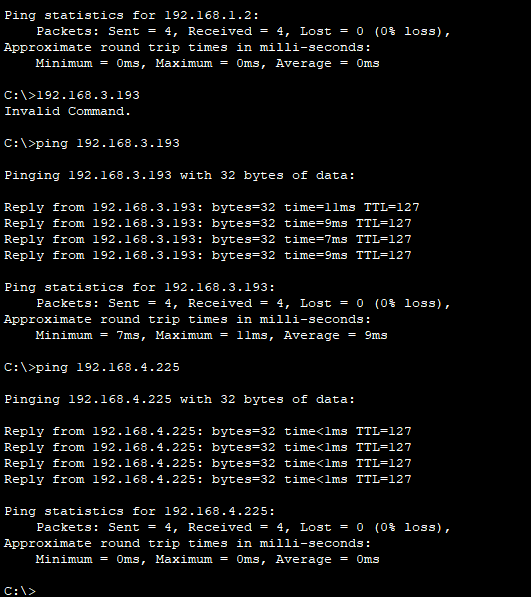
\includegraphics[scale=0.36]{P1/img/datatupen1.png}
        \caption{Koneksi antar PC Sederhana Menggunakan Cisco}
        \label{fig:tupenp1}
    \end{center}
\end{figure}

	\item Tabel Routing Sederhana
\begin{table}[h]
    \centering
    \caption{Tabel Routing Jaringan}
    \label{tab:tabel_routing}
    \begin{tabular}{|c|c|c|c|}
    \hline
    \textbf{Network Destination} & \textbf{Netmask/Prefix} & \textbf{Gateway} & \textbf{Interface Tujuan} \\
    \hline
 	192.168.1.0 & 255.255.255.128 (/25) & 192.168.1.1 & FastEthernet0/1 (RnD) \\
    192.168.2.128 & 255.255.255.128 (/25) & 192.168.2.128 & FastEthernet0/0 (Produksi) \\
    192.168.3.192 & 255.255.255.224 (/27) & 192.168.3.192 & FastEthernet1/0 (Administrasi) \\
    192.168.4.224 & 255.255.255.240 (/28) & 192.168.4.224 & FastEthernet1/1 (Keuangan) \\
    \hline
    \end{tabular}
\end{table}
\item Routing yang sesuai dengan perusahaan
Dapat menggunakan Static Routing untuk perusahaan ini karena kebutuhan jaringan yang relatif kecil. Perusahaan ini hanya memiliki empat departemen dengan jumlah perangkat yang terbatas, sehingga Static Routing lebih efisien daripada Dynamic Routing. Dengan Static Routing, konfigurasi rute dilakukan secara manual, yang membuatnya lebih mudah diterapkan pada jaringan sederhana seperti ini.
Keuntungan lain dari Static Routing adalah keamanannya. Karena rute ditentukan secara manual, kita memiliki kontrol penuh atas jalur yang digunakan oleh data, sehingga mengurangi risiko perubahan otomatis yang bisa disebabkan oleh protokol routing dinamis.
Secara keseluruhan, Static Routing adalah pilihan yang tepat karena lebih mudah diterapkan, memberikan kontrol penuh, dan cukup untuk memenuhi kebutuhan perusahaan yang memiliki jaringan kecil dan stabil. Jika perusahaan berkembang besar di masa depan dapat mempertimbangkan Dynamic Routing.
\end{enumerate}